\documentclass[10pt,a4paper]{book}
\usepackage[latin1]{inputenc}
\usepackage{amsmath}
\usepackage{amsfonts}
\usepackage{amssymb}
\usepackage{graphicx}
\usepackage{tikz}
\author{Cano Jones, Alejandro}
\title{Problemas de Fundamentos de la F�sica II}
\date{Curso 2017-2018}
\begin{document}
	\maketitle
	\tableofcontents
	\section{Campos Conservativos}
	\subsection{Ejercicio 1}
	\paragraph{Enunciado:} Tres cargas puntuales $q = 3\cdot10{-9} [C]$ se sit�an en tres de los v�rtices de un cuadrado de lado $L = 15 cm$. Determina el campo el�ctrico (m�dulo y orientaci�n) en el v�rtice vacante.
	\paragraph{Realizaci�n:}
	\begin{center}
		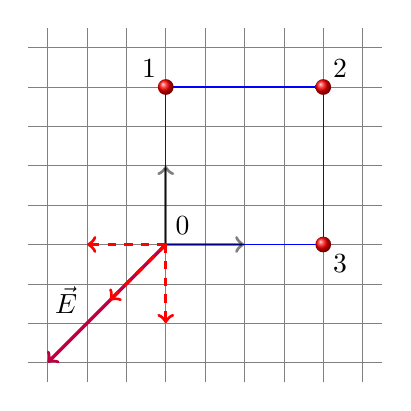
\begin{tikzpicture}
			\draw[step=0.5cm,gray,very thin] (-1.75,-1.75) grid (2.75,2.75);
			\draw [blue] (0,0) rectangle (2,2);
			\draw [very thick, opacity=0.5] [->] (0,0)--(0,1);
			\draw [very thick, opacity=0.5] [->] (0,0)--(1,0);
			\draw [very thick, dashed, red] [->] (0,0)--(-1,0);
			\draw [very thick, dashed, red] [->] (0,0)--(0,-1);
			\draw [very thick, purple] [->] (0,0)--(-1.5,-1.5);
			\draw [very thick, dashed, red] [->] (0,0)--(-0.71,-0.71);
			\shade [ball color=red] (0,2) circle (0.1);
			\shade [ball color=red] (2,2) circle (0.1);
			\shade [ball color=red] (2,0) circle (0.1);
			\node [above right] at (0,0) {0};
			\node [above left] at (0,2) {1};
			\node [above right] at (2,2) {2};
			\node [below right] at (2,0) {3};
			\node [above left] at (-1,-1) {$\vec{E}$};
		\end{tikzpicture}
	\end{center}
	Tal como se ha representado en la figura, el campo generado por las particulas es repulsivo (puesto que las cargas son positivas).
	Sabemos por el principio de superposici�n de campos, que el valor del campo en un punto dado es igual a la suma de los valores de los campos existentes; por ello, comenzamos describiendo los campos:
	\begin{equation}
		\vec{E_1}=-K\frac{q}{L^2} \hat{j} \left[\frac{N}{C}\right]
	\end{equation}
	\begin{equation}
	\vec{E_2}=-K\frac{q}{L^2} \hat{i}-K\frac{q}{L^2} \hat{j} \left[\frac{N}{C}\right]
	\end{equation}
	\begin{equation}
	\vec{E_3}=-K\frac{q}{L^2} \hat{i} \left[\frac{N}{C}\right]
	\end{equation}
	A continuaci�n, solo debemos sumar todos los valores:
	\begin{equation}
		\vec{E}=\sum_{i=1} \vec{E_i}=-2K\frac{q}{L^2} \hat{i}-2K\frac{q}{L^2} \hat{j}\left[\frac{N}{C}\right]
	\end{equation}
	
	Tomando los valores $K=8.99\cdot 10^9 \left[\frac{Nm^2}{C^2}\right]$ (Suponiendo el sistema se encuentre en el vac�o) y $L=0.15m$, operamos y obtenemos:
	\begin{equation}
	\vec{E}=-2.397\cdot 10^3\hat{i}-2.397\cdot 10^3 \hat{j}\left[\frac{N}{C}\right]
	\end{equation}
	Donde el m�dulo ser� $|\vec{E}|=2.397\cdot 10^3\cdot\sqrt{2}\left[\frac{N}{C}\right]$ formando un �ngulo de $\frac{3}{2}\pi\left[rad\right]$ tal como se muestra en la figura.
	
	\subsection{Ejercicio 2}
	\paragraph*{Enunciado:}
	Una masa $m$ est� situada a una distancia $z$ del centro de un disco delgado de masa $M$ y radio $R$. Determina la fuerza de atracci�n gravitatoria entre la masa y el disco.
	\paragraph{Realizaci�n:}
	
	\subsection{Ejercicio 3}
	\paragraph{Enunciado:}
	En un plano homog�neo e indefinido, con masa por unidad de superficie $\sigma$, se recorta y retira un trozo circular de radio $R$. Determina el campo y el potencial gravitatorios en los puntos a lo largo de un eje perpendicular al plano y que pasa por el centro del agujero.
	\paragraph{Realizaci�n:}
	\begin{center}
		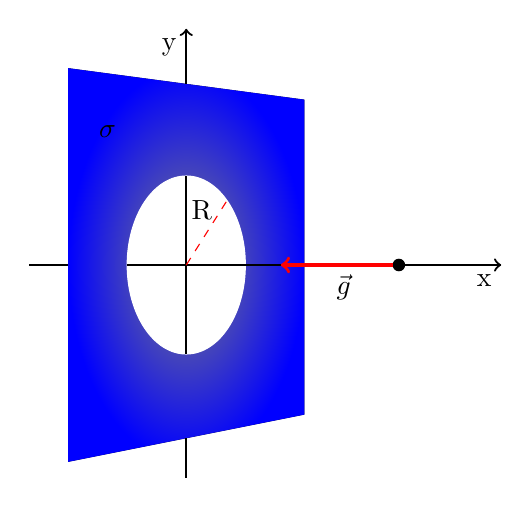
\begin{tikzpicture}
			\fill [outer color=blue] (-1.5,-2.5)--(1.5,-1.9)--(1.5,2.1)--(-1.5,2.5)--cycle;
			\draw [fill, color=white](0,0) ellipse (0.75cm and 1.13cm);
			\draw [thick] [->] (-0.75,0)--(4,0);
			\draw [thick] (0,-1.13)--(0,1.13);
			\draw [thick] [->] (0,2.3)--(0,3);
			\draw [thick] (-1.5,0)--(-2,0);
			\draw [thick] (0,-2.2)--(0,-2.7);
			\draw [dashed, red] (0,0)--(0.55,0.87);
			\fill [black] (2.7,0) circle (0.08);
			\draw [very thick, red] [->] (2.62,0)--(1.2,0);
			\node at (-1,1.7) {$\sigma$};
			\node [below] at (2,0) {$\vec{g}$};
			\node [below left] at (0,3) {y};
			\node [below left] at (4,0) {x};
			\node [above left] at (0.45, 0.45) {R};
		\end{tikzpicture}
	\end{center}
	Sabemos por el principio de superposici�n de campos, que el valor del campo generado por varias particulas es igual a la suma del campo generado por cada particula individual. A su vez, conocemos el valor del campo generado por un plano infinito y el valor del campo generado por un disco; es por ello, que podemos calcular el campo generado por esta estructura sustrayendo el valor del campo generado por un disco al campo generado por el plano, esto es:
	\begin{equation}
		\vec{g}=\vec{g}_{Plano}-\vec{g}_{Disco}=\left(-G 2\pi\sigma\right)\hat{i}-\left[-G 2\pi\sigma\left(1-\frac{1}{\sqrt{1+\left(\frac{R}{x}\right)^2}}\right)  \right]\hat{i}\left[\frac{N}{C}\right]
	\end{equation}
	Operando, llegamos al resultado:
	\begin{equation}
		\vec{g}=-G\frac{2\pi\sigma}{\sqrt{1+\left(\frac{R}{x}\right)^2}}\hat{i}\left[\frac{N}{C}\right]
	\end{equation}
	\subsection{Ejercicio 4}
	\paragraph{Enunciado:}
	Calcula el campo gravitatorio en los puntos $A$ y $B$ de la distribuci�n de masa de la figura, en la que se muestra una esfera de radio $2R$ y densidad $\rho$, en cuyo interior existe una cavidad esf�rica de radio $R$ llena de un material de densidad $\rho$.
	\paragraph{Realizaci�n:}
\end{document}

